\documentclass[]{report}
\usepackage{graphicx}
\usepackage{caption}
\usepackage{refstyle}
\usepackage{blindtext}
\usepackage[utf8]{inputenc}
\usepackage{csvsimple}

% Title Page
\title{Research Application Development Frameworks for Java Enterprise Development \newline and Develop JEE Prototype with Framework}
\author{David Kelly}


\begin{document}
\maketitle

\newpage

\section{Project Overview}

	\subsection{Project Title}
	Research Application Development Frameworks for JEE Development, and Develop JEE Prototype with Framework
	
	\subsection{Project Type}
	Research and JEE Prototype application
	
	\subsection{Project Client}
	Institute of Technology Blanchardstown
	
	\subsection{Project Supervisor}
	Geraldine Gray
	
	\subsection{Project Manager}
	David Kelly
	
	\subsection{Project Timescale}
	14/9/2015 - 30/4/2016

	\section{Executive Summary}
	This proposal explores the potential to incorporate JEE compatible frameworks in to application development to reduce the development time and increase the application performance. 
	
	This proposal introduces what frameworks are and how they can be implemented. In order to choose the correct framework to implement in JEE app development it is important to research what components the framework manages.
	
	This proposal suggests learning about \underline{four} potential frameworks and building a prototype application with \underline{one} of the frameworks.
	
	A successful project would analyze cost, time, compare frameworks and examine their implementation within a JEE environment.

\newpage

\section{Introduction}

The aim of this project is to research four popular Java Enterprise Edition compatible frameworks and develop a JEE prototype application from one of the researched frameworks. The Java EE platform provides an API and runtime environment for developing and running large-scale, multi-tiered, scalable, reliable, and secure network applications [1]. With many multifaceted components making up a JEE application it is easy for a developer to be obstructed from creating the application they wish and can find themselves bogged down in the technical processes of simply getting the application to function. 

A framework’s primary purpose is to aid and ease an applications development process. It should allow for an application to develop quickly and easily and should result in a superior finished application [2]. Upon researching these frameworks, I will evaluate their core features and analyzing how each framework is suited to be implemented within a JEE application.


I will develop a JEE prototype application using one of the frameworks I feel can further my understanding. While developing the application I will document and compare how the framework provides an advantage over the standard Java API, further I will asses the learning curve involved with implementing the chosen framework.

	\subsection{Background}
	Frameworks have been around since the release of J2EE (Java 2 Enterprise Edition) in late 1999. Struts framework was created by Craig McClanahan (later donated to Apache Foundation) to improve the development experience over pure Java Server Pages (JSP) utilization [3]. With the many updates and releases of what is now known as simply JEE (Java Enterprise Edition) so too came many frameworks looking to improve on standard JEE components. 
	
	Frameworks accommodate developers who do not have specific knowledge of all components of JEE application development. The ability to plugin a framework to a project can reduce overhead related to app development. Modern developers do not need to specialize in persisting data, database management, management of dependencies, security. Developers can simply select a framework that can manage these components and write programs that utilize these framework classes.
	
	Choosing the correct framework to develop a JEE application can be difficult and there is no single correct answer. This project proposes to find out what popular current frameworks exist for JEE and when they should be incorporated in to a JEE project. 
		
\newpage
		
	\subsection{Existing Technologies}
	In order to select the frameworks to be researched we must look at some of the existing and more popular frameworks for JEE. 
	
	In May 2014 software development community www.zeroturnaround.com [4] commissioned a survey to find out what Java frameworks are most used by current developers. The survey was carried out on 2164 Java developers. The results are shown in figure 3.1
	
		\begin{figure}[h]
			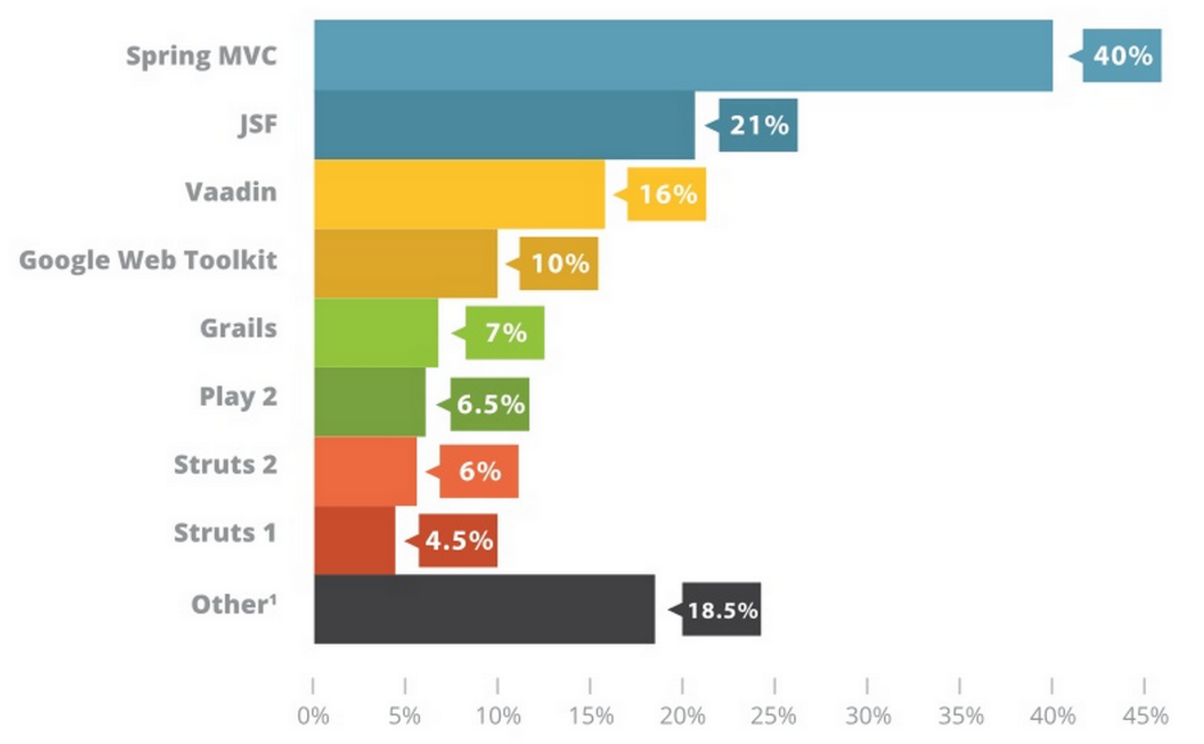
\includegraphics[width=.7\textwidth]{img1.png}
			\begin{center}
			\figurename{ 3.1}
			\end{center}
		\end{figure}
		
		In Nov 2014 software developer blog www.vitalflux.com [5] conducted a survey of the most sought after positions in JEE framework development. Figure 3.2.			

		\begin{figure}[h]
			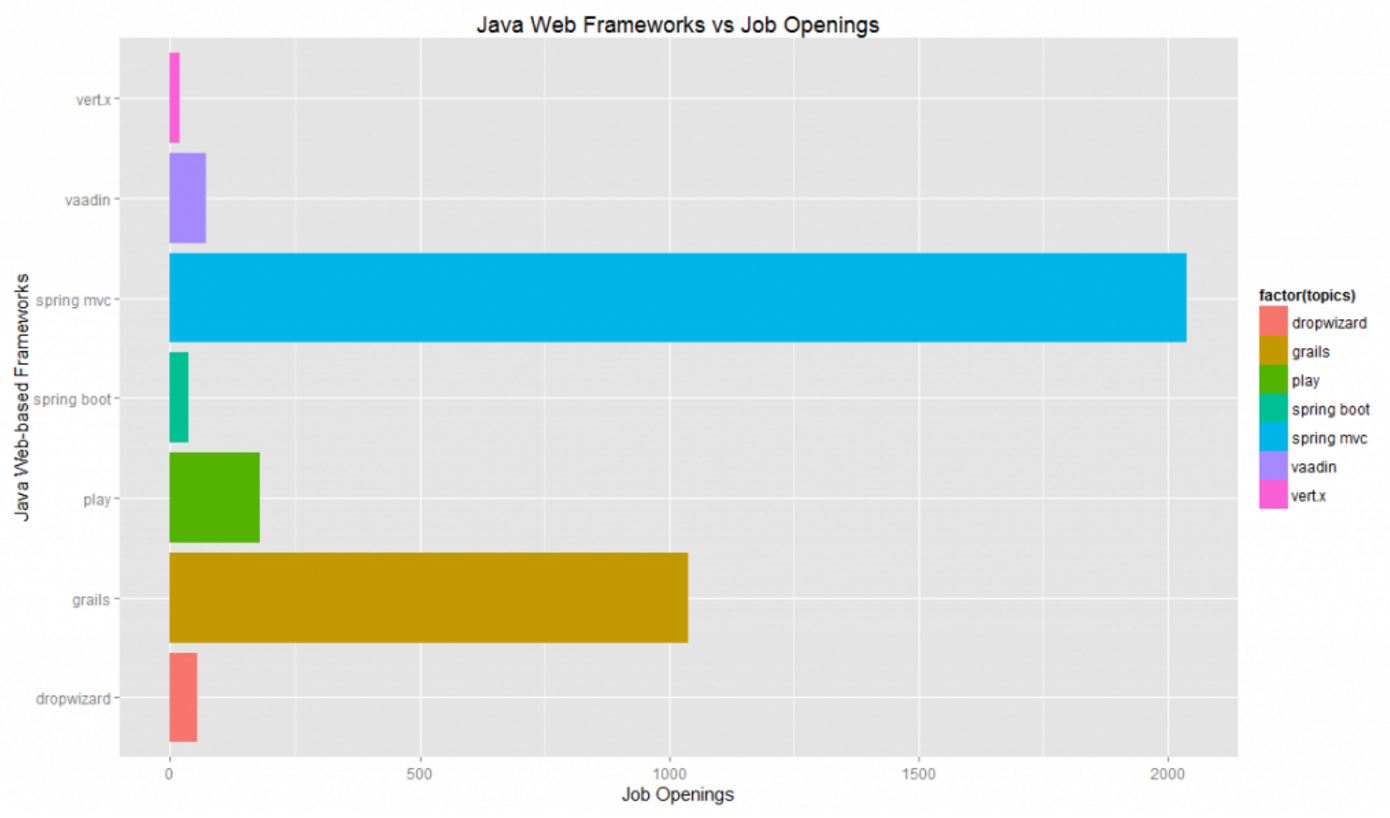
\includegraphics[width=.7\textwidth]{img2.png}
			\begin{center}
				\figurename{ 3.2}
			\end{center}
		\end{figure}

\newpage

	These websites are not the final say on the community of Java framework developers or the professional market that use frameworks. these surveys are good indications of what frameworks are popular, have large communities and are established in the current developer environment.
	
	In choosing the frameworks to study I would lean toward cross referencing both of the surveys above and selecting frameworks present and well represented in both. 

\section{Main Research Question}
	\subsection{Does the choice of framework affect the application?}
	With many different standardized frameworks available to incorporate into a JEE project, can the choice of framework impact the performance of the final application? 
	\subsection{Can a project accommodate a frameworks learning curve?}
	Mastering a framework comes with a cost, is it worth learning an entire framework for a single project?
	\subsection{Can frameworks be compared?}
	What are there commonalities between frameworks that allow them to be compared?
	\subsection{What are the major differences between the researched frameworks?}
	From the four frameworks researched what area of application development to they best suit? 
	\subsection{Can one of the researched frameworks be implemented in a project}
	Can a prototype JEE application be developed to display the abilities of the chosen framework?

\newpage

\section{Benefits}
	\subsection{Developer Benefits}
	Understanding of existing frameworks\newline
	Knowledge of existing frameworks allow a developer to plan a project while incorporating a framework that can manage a component of the application. Understanding what frameworks do and how they can be utilized increases a developers’ ability to create applications. Researching four frameworks will give a strong foundation on what frameworks are, what they do, how they can be incorporated and when. 

	Critical ability to compare features of frameworks\newline
	Critical analysis of frameworks and their features will be a benefit. Becoming familiar with frameworks and how they are comprised and implemented can further the ability of a developer to build an application employing the correct framework with maximum impact with the smallest overhead. It is not necessary to have large amounts of classes that are unimplemented if only few classes are needed  

	Learning how to develop with chosen framework while building prototype\newline
	After choosing the framework to develop the JEE prototype, the developer will learn valuable skills regarding the implementation of the framework. Using and IDE and downloading the plugin and classes needed then learning about the modules available to create a complete JEE application.

	
	\subsection{Project Benefits}
	Ability to develop application faster\newline
	Correctly implementing the framework in to the prototype project should accelerate application development while increasing the functionality of the final application.
	
	Example of chosen framework in prototype application\newline
	Upon completion of this project an example application created with a chosen framework should show the capabilities and improvements possible when incorporating the correct framework in to the JEE application

	Knowledge of other frameworks that have potential use\newline
	While this project intends to use one of the researched frameworks to create a prototype application, It is possible to incorporate multiple frameworks in to a single project. Knowing what frameworks can do will benefit the projects ability to incorporate more than one if extended or upon removal and replacement of existing framework.
	
	\subsection{Future Benefits}
	Creating a prototype application will show the capabilities of the framework. Further mastering of the chosen framework can be used on larger projects in future. After the initial cost of the learning curve for the first project, future project development will be quicker and can use other frameworks touched upon in research project.

\section{Feasibility}
	\subsection{Technical Requirements}
	In order to undertake this project it is required that the lead role has experience with Java and has previously worked on projects of similar size. Researching four unique Java frameworks will require library resources and an aptitude for developing and learning simultaneously. The knowledge of a Java IDE is necessary and access to download plugins needed. A working understanding of JEE applications is required as the prototype will be developed in a JEE environment.  
		
	The project has a fixed timeframe marked with frequent deliverables and meetings to assess project progression.

	I have worked on projects in the past developing applications through many different Java IDE's. I have produced documents and literature on topics such as Java GUI design, web based games built with PHP and I have spent 3 years developing with Java. I am currently studying in Institute of Technology Blanchardstown and have college access to resources including, computer labs, library resources and a project supervisor (MSc Geraldine Gray).

\section{Proposed Methodologies}
	\subsection{Researching existing Java frameworks}
	A literature review will be carried out on four of the chosen frameworks. The purpose of this literature review is to understand and become familiar with the features of each framework. Access to existing projects through public GitHub repositories can provide information on Java projects that use these frameworks and how other developers have incorporated them in to their applications. Researching current websites that implement Java frameworks will show a working environment of what each framework is capable of doing.
	
	
	\subsection{Comparing frameworks}
	Comparing characteristics of frameworks is a bases for overall understanding of their core features. Comparing the size of the framework plugin classes, The impact the framework has on the existing Java code, The learning curve involved in working with a framework, the removal of a framework from a project, how a framework manages dependencies, community support for the framework.

\newpage	

	\subsection{Prototype Implementation}
	The prototype JEE application should with developed with the waterfall SDLC model. 

		\begin{figure}[!htb]
			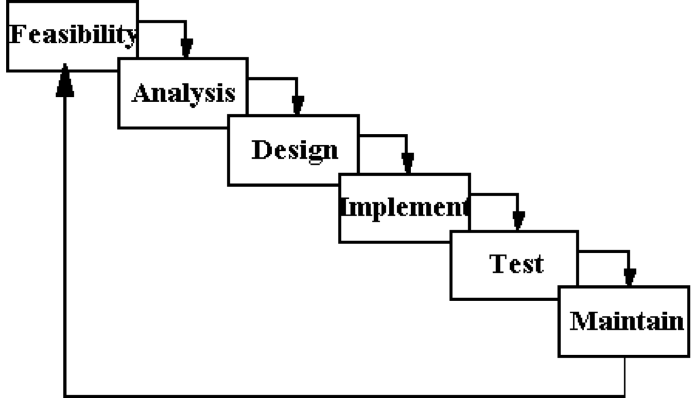
\includegraphics[width=.8\textwidth]{img3.png}
			\begin{center}
				\figurename{ 7.3}
			\end{center}
		\end{figure}
			
	\subsubsection{Advantages}
	\begin{itemize}
		\item Simple and easy to understand and use.
		\item Easy to manage due to the rigidity of the model – each phase has specific deliverables and a review process.
		\item Phases are processed and completed one at a time.
		\item Works well for smaller projects where requirements are very well understood.
	\end{itemize}
	
	\subsubsection{Disadvantages}
	\begin{itemize}
		\item Difficult to move back stages
		\item No working software is produced until late during the life cycle.
		\item Poor model for long and ongoing projects.
	\end{itemize}

\newpage

\section{Expected Results}
	\subsection{Successful Research}
	Successfully researching all frameworks will entail the lead researcher developing a firm understanding of each individual framework. Becoming familiar with the characteristics of the framework, critically being able to compare each individual framework and distinguishing their abilities within a JEE application. The research phase of the project should deliver the framework to be used in developing the prototype. Knowing what JEE application to be developed and how the framework will improve the development.
	
	\subsection{Successful Application}
	A successful implementation of the JEE prototype application should incorporate one of the four researched java compatible frameworks. The application will be fully functional with all components of a JEE application fully involved some at least one of which managed by the framework. The final version of the prototype will be submitted before the deadline on the 30/4/2016.
	
	\subsection{Successful Project}
	In order for the project to be considered successful, the research should improve the researcher's knowledge of Java compatible frameworks. Four frameworks in particular should be known with great detail. One of the frameworks should be used to develop a prototype application that displays the capabilities of the framework within a JEE environment application.
	
	The entire development process need to be documented with industry standard code and a .war file that can be deployed on a Java server as a standalone.
	
	\subsection{Failed Project}	
	A failed project can occur if the research phase does not correctly investigate four Java compatible frameworks. If the research process is too vague and knowledge of frameworks is not documented correctly. 
	
	The ability to create a prototype JEE application may not be hindered by the lack of research. How ever without a complete research phase to support the reasoning and choice of framework used to develop the prototype app the application will be considered unsuccessful. Should the final prototype application not be submitted before the deadline date, the project will also be considered unsuccessful. 

\newpage

\section{Conclusion}
	In order to begin the next phase of the project it is important to understand the most important concepts of this proposal.
	
	\begin{enumerate}
		\item The project should center on the research of \underline{four} Java EE compatible frameworks.
		\item All unique features of each framework should be assessed and all commonalities compared.
		\item After researching the frameworks, \underline{one} should be chosen to develop in a complete prototype JEE application.
		\item The prototype should follow the waterfall SDLC with frequent reviews from the project supervisor.
		
	I have the ability and resources available to complete this project within the allocated timeframe following the timeline and gannt chart proposed. 
	\end{enumerate}

\section{References}
	\begin{enumerate}
		\item Oracle. 2015. Oracle JavaEE. [ONLINE] Available at: \newline https://docs.oracle.com/javaee/6/firstcup/doc/gkhoy.html. [Accessed 23 October 15].
		\item Michael Nash, 2003. Java Frameworks and Components: Accelerate Your Web Application Development. Edition. Cambridge University Press. pg12
		\item Struts. 2015. Apache Struts End Of Life [EOL]. [ONLINE] Available at:
		http://struts.apache.org/struts1eol-press.html. [Accessed 21 October 15].
		\item ZeroTurnAround. 2014. Top 4 Java web frameworks revealed. [ONLINE] Available at: http://zeroturnaround.com/rebellabs/top-4-java-web-frame works-revealed-real-life-usage-data-of-spring-mvc-vaadin-gwt-and-jsf/. \newline
		[Accessed 22 October 15]
		\item Vitalflux. 2014. Java - Top 10 Java-based frameworks 2014-2015. [ONLINE] Available at: http://vitalflux.com/java-top-10-java-based-web-dev \newline elopment-frameworks-2014-2015/ [Accessed 22 October 15]
	\end{enumerate}

\newpage

\section{Project Plan}
	\subsection{Project table}
	\csvautotabular{projecttime.csv}

\newpage

	\subsection{Gannt Chart}
		\begin{figure}[!htb]
			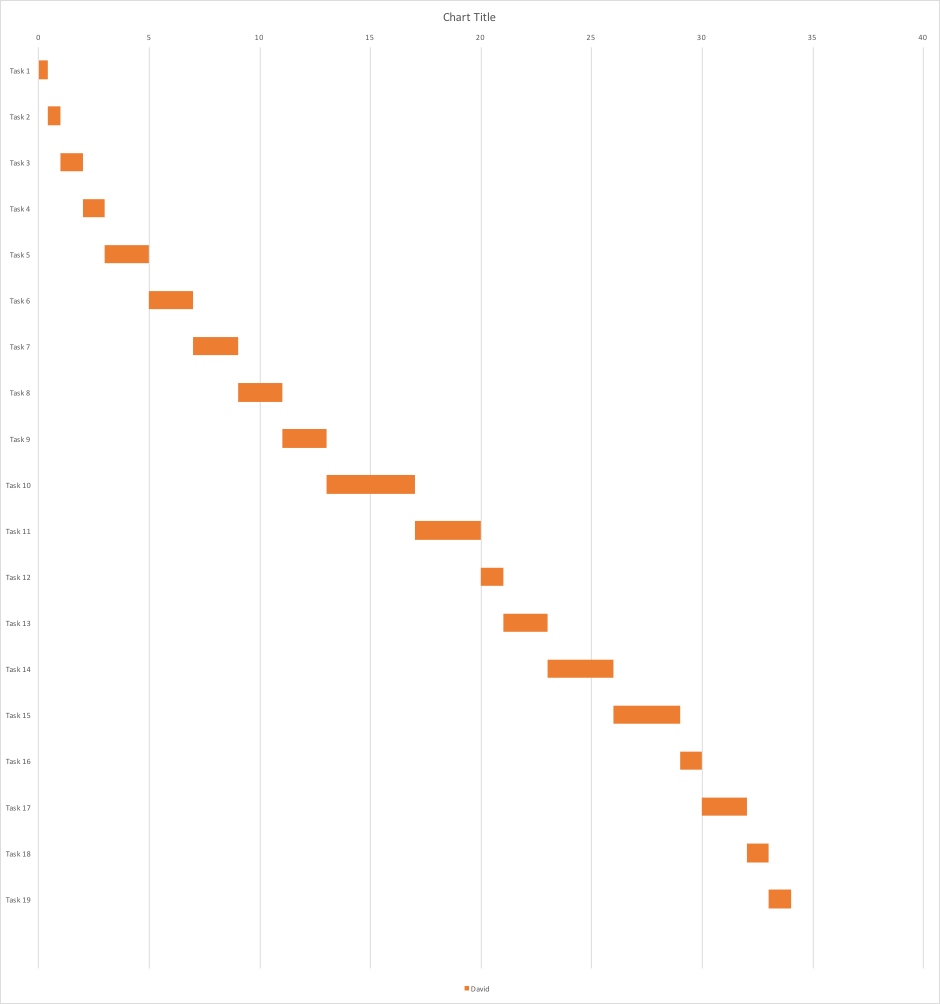
\includegraphics[width=\textwidth]{img4.png}
			\begin{center}
				\figurename{ 11.1}
			\end{center}
		\end{figure}

\end{document}          
